
\documentclass{acm_proc_article-sp}

\usepackage{amsmath}
\usepackage{verbatim}
\usepackage{textcomp}
\usepackage{graphicx}
\usepackage{subcaption}
\usepackage{url}


\begin{document}

\title{Difficult Handwritten Digit Classification \\
{\normalsize Code available at: \url{https://github.com/slflmm/Miniproject-3}}} 
\subtitle{COMP 598 -- Miniproject 3 -- Team X}

\numberofauthors{3} 
\author{
% 1st. author
\alignauthor 
Narges Aghakazemjourabbaf\\
	\affaddr{?}
\alignauthor
Stephanie Laflamme\\
	\affaddr{260376691}
% 2nd. author
\alignauthor Benjamin La Schiazza\\
	\affaddr{?}
% 3rd. author
}

\date{Oct15}



\maketitle
\begin{abstract}

\end{abstract}

\section{Introduction}% overview of approach

\section{Preprocessing}
Standardization (x-mean/standard deviation)
Contrast normalization

\section{Feature Design and Selection}
When appropriate for the learner, we consider three feature sets; raw pixels, PCA, and Gabor filter-based features.

\subsection{Pixels}
We use the post-standardization pixel information as a baseline feature set.This produces feature vectors of length 2304. 

\subsection{PCA}
(Describe PCA)

As removing the least useful features made the results of our baseline classifier worse, we keep the same initial number of dimensions. 

\subsection{Gabor}
\cite{Bau}

\section{Algorithm Selection}% for each category
\subsection{Perceptron}

\subsection{Neural Network}

\subsection{Linear SVM}
Use Scikit-learn implementation \cite{scikit-learn}

\subsection{Convolutional Neural Network}
Origin of convnets \cite{Fukushima}. We can see it has good invariance to rotation and resistance to noise with the MNIST dataset. \cite{LeCun}

Problem of neural networks = overfitting. Regularization... (L1 + L2 norms). Dropout \cite{Hinton}
Dropout in fully-connected layers of a convolutional net \cite{Krizhevsky}
SGD with minibatches.
Momentum.


\section{Optimization} % if required
GPU for convolutional network -- Theano \cite{Theano}

\section{Parameter Selection Method}% model order, learning rate, etc
Preliminary manual search followed by either:

Gridsearch 

Random search \cite{Bergstra}

\section{Testing and Validation}%detailed analysis of results

\subsection{Perceptron}
In a primary step, we performed 5-fold cross-validation to compare raw pixels, PCA, and Gabor features using a fixed learning rate ($\alpha = 0.01$) and number of iterations (15). As shown in Table \ref{tab:perc-features}, the most performant feature set was ???, with a validation accuracy of ????.
\begin{table}[h!]
  \centering
  \begin{tabular}{|c||c|c|c| }
    \hline
    Features & Pixels & PCA & Gabor \\
    \hline
    Accuracy & 25.794 & 26.282 & 10 \\
    \hline
  \end{tabular}
  \caption{Mean validation accuracy of perceptron using different features}
  \label{tab:perc-features}
\end{table}

Using (the best feature set), we performed 5-fold cross-validation over the learning rate $\alpha$ and the number of training iterations of the perceptron model. Figure \ref{fig:perc-gridsearch} shows the results of gridsearch with both parameters. The precise values of the best parameters found by the gridsearch cross-validation procedure were $\alpha = 0.0005$ with 20 training iterations, yielding a mean validation accuracy of 26.594\%.\footnote{Additional results showing training error vs validation error are shown in Appendix 1}
\begin{figure}[h!]
	\centering
	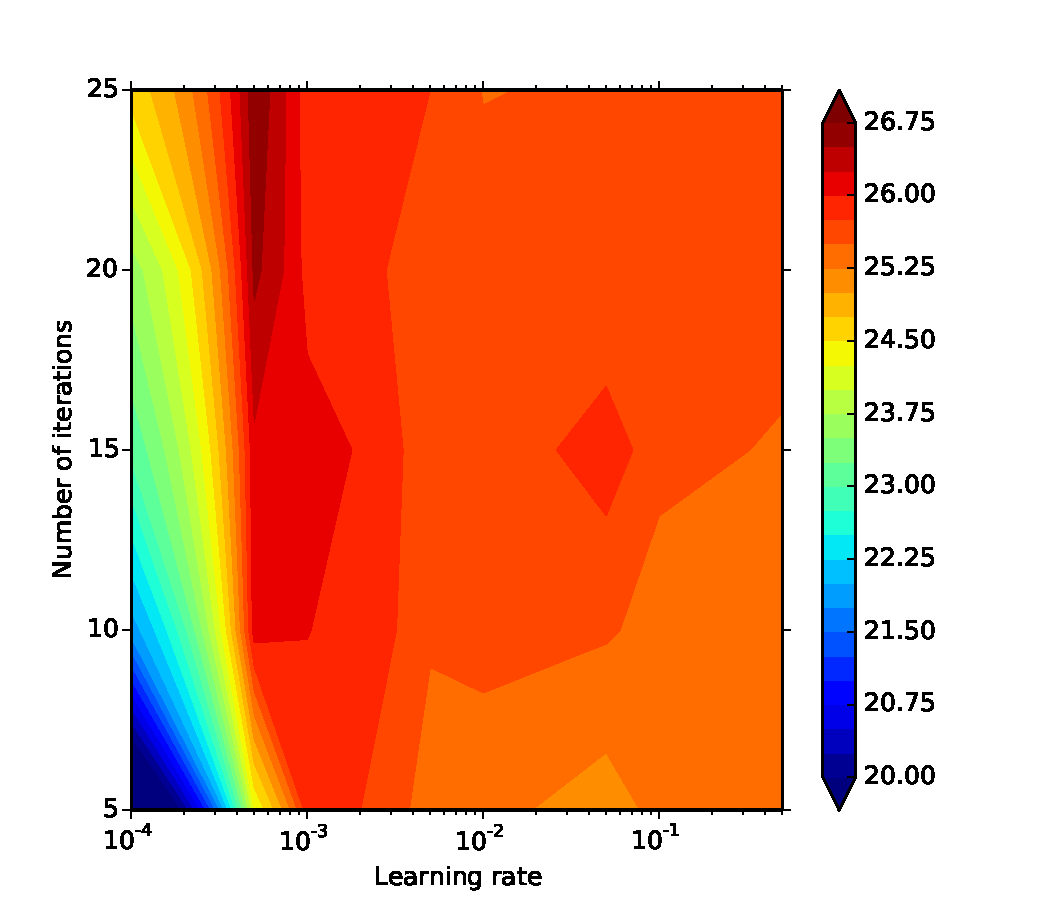
\includegraphics[width=\linewidth]{perceptron_gridsearch}
  	\caption{Mean cross-validation accuracy as a function of parameters $\alpha$ and number of iterations}
  	\label{fig:perc-gridsearch}
\end{figure}

After training our perceptron on the complete training set using these parameters, we submitted our results to Kaggle and obtained a test accuracy of ???. As an approximation of the test confusion matrix, we provide the confusion matrix for the combined validation sets in Figure \ref{fig:perc-confusion}. Note the perceptron's greater ability to identify 0s and 1s compared to other digits.
\begin{figure}[h!]
	\centering
	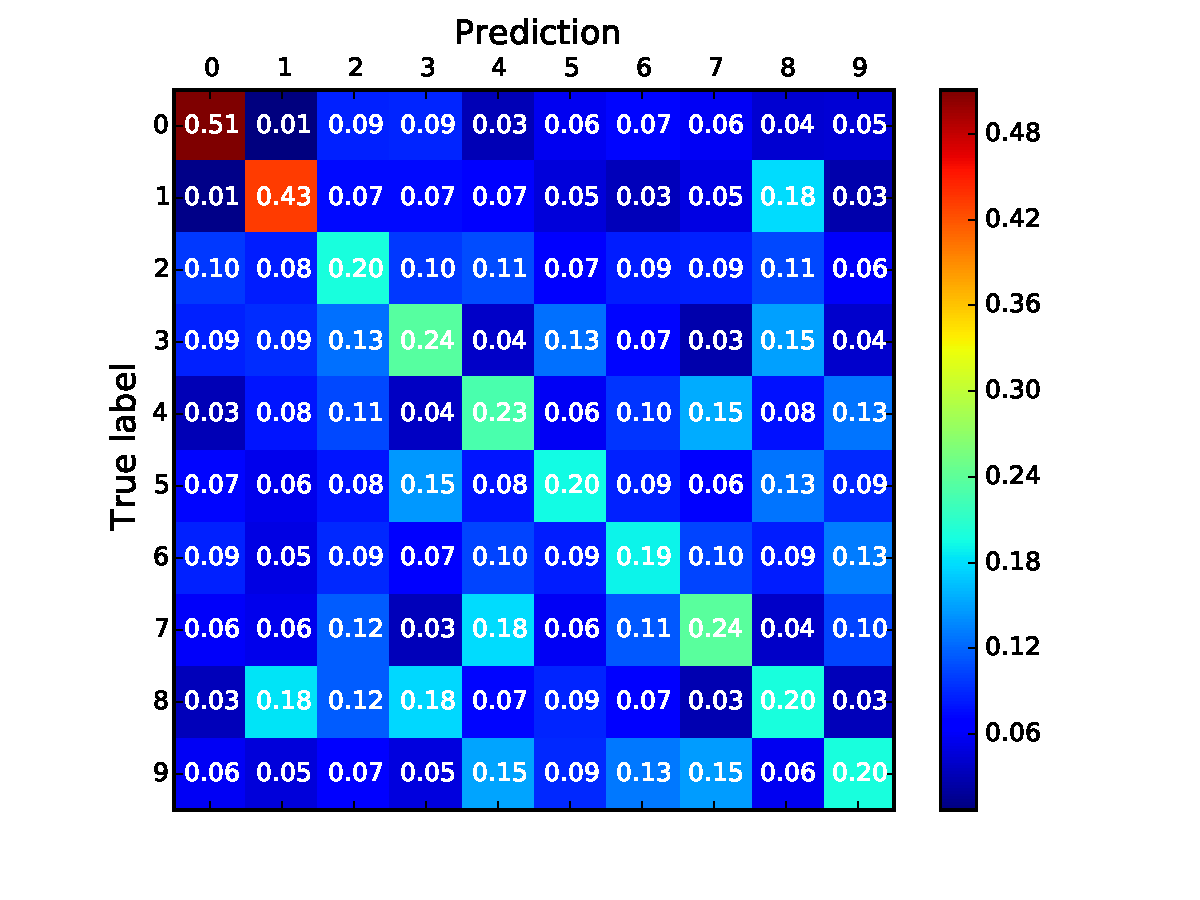
\includegraphics[width=\linewidth]{perceptron_confusion}
  	\caption{Validation confusion matrix for perceptron}
  	\label{fig:perc-confusion}
\end{figure}

\section{Discussion}% pros/cons of approach & methodology (and alternatives)
Why is it better at classifying 0s and 1s? (Check number of examples in classes--could be Benford's law?

Using Gabor filters as a kernel rather than feature \cite{Sabri}

Other version of dropout \cite{Wan}

Pretraining \cite{Erhan}

Others: \cite{Rowley}, \cite{Simard}

{\bfseries We hereby state that all the work presented in this report is that of the authors.}

\bibliographystyle{abbrv}
\bibliography{references}

\appendix

\section{Additional results}
\begin{figure}[h!]
	\centering
	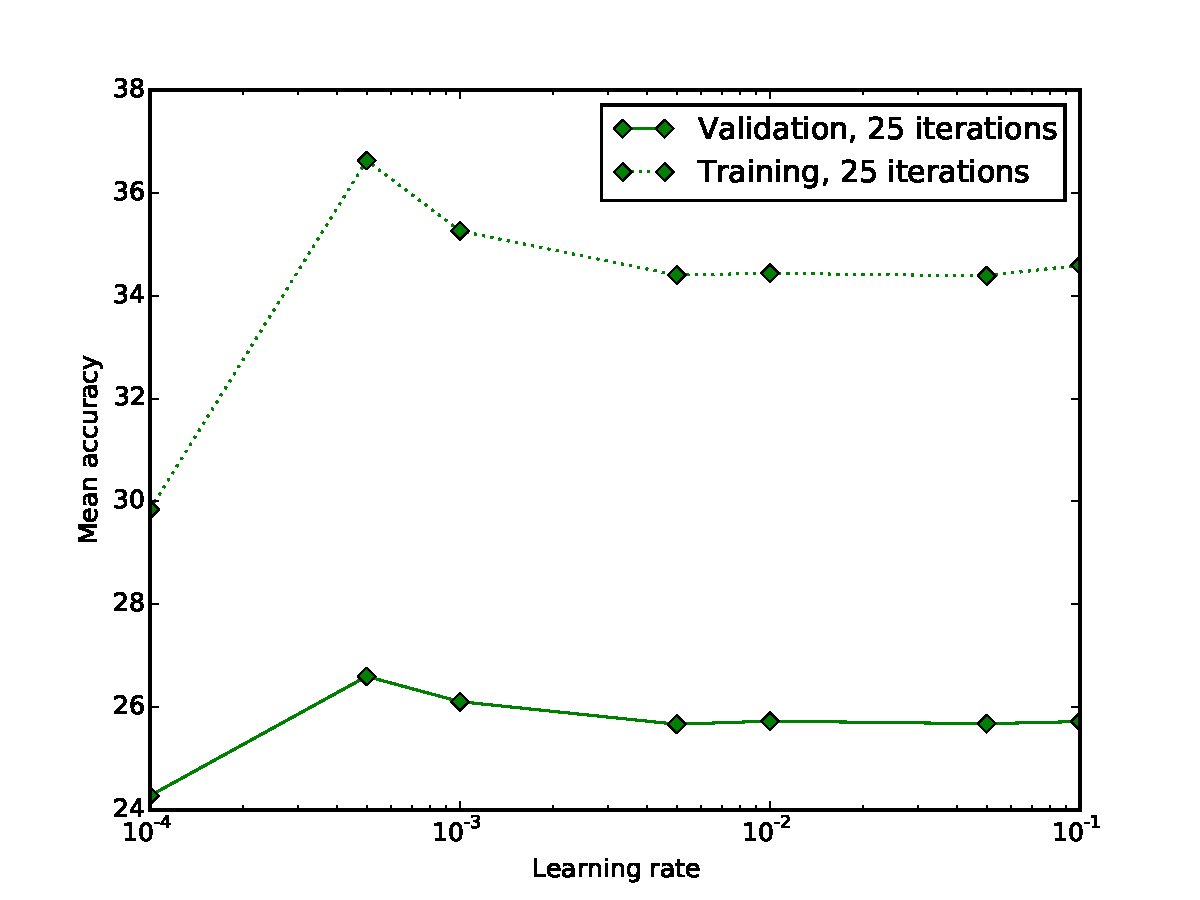
\includegraphics[width=\linewidth]{perceptron_learningrate}
  	\caption{Cross-validation over $\alpha$ with perceptron, keeping \# iterations optimal}
  	\label{fig:perc-learningrate}
\end{figure}
\begin{figure}[h!]
	\centering
	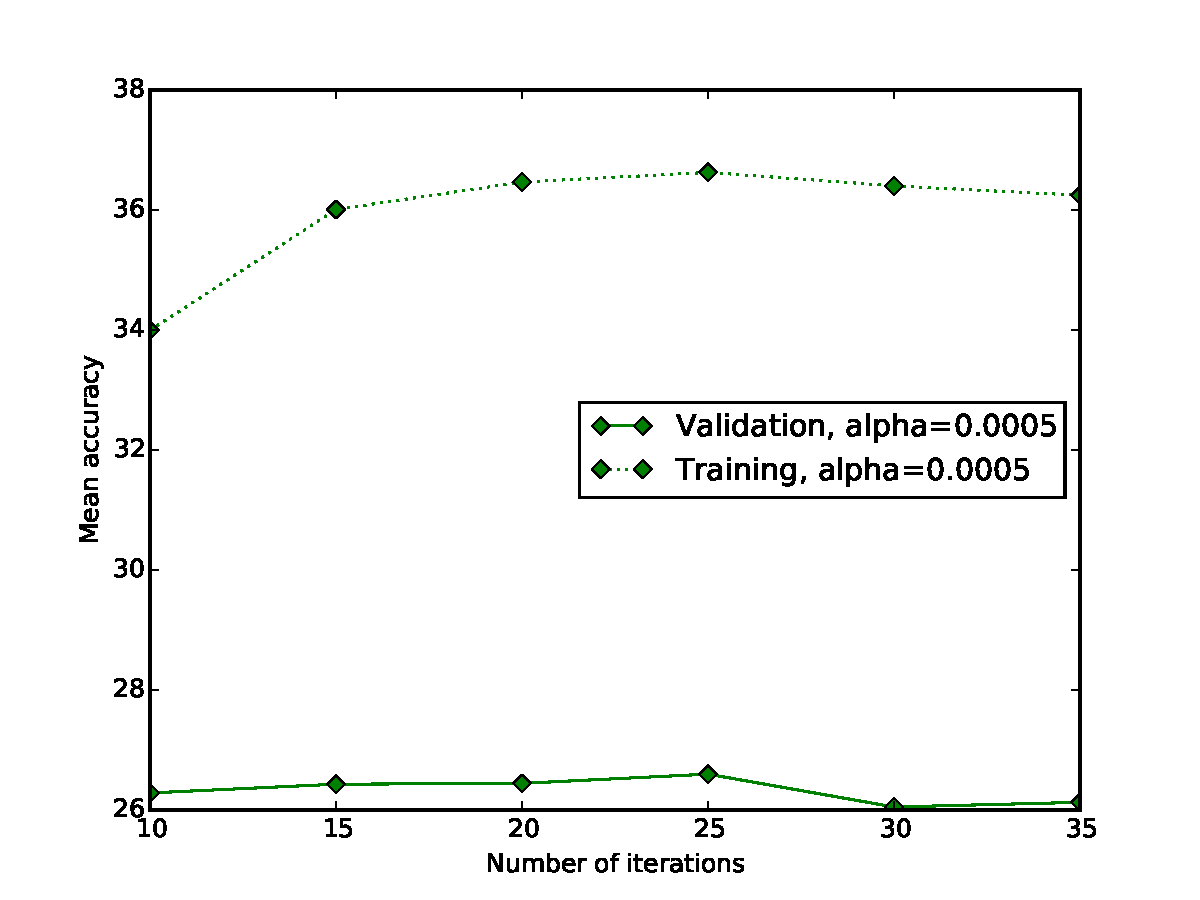
\includegraphics[width=\linewidth]{perceptron_iterations}
  	\caption{Cross-validation over \# of iterations with perceptron, keeping $\alpha$ optimal}
  	\label{fig:perc-iterations}
\end{figure}


\balancecolumns
\end{document}